In the previous sections, we discussed about the anatomy of the brain and neurons and how studies indicate that these cells might communicate via electrochemical pulses known as action potentials or \emph{spikes}. It's known that sensory input is somehow encoded so that the brain can process it, the exact encoding is not yet known and is the subject of active research effort. Similarly, how is the brain able to reconstruct (or decode) prior input from action potentials is an open question. The so called \emph{neural code} is one of the most important questions in neuroscience and different hypotheses have been proposed, some of which are described bellow~\cite{dayan2001theoretical,gollisch2009throwing}.

\subsection{Rate code}
Spike-rate encoding, in its simplest case, represents information with the amount of action potentials that a neuron generated in a time interval. It is one of the earliest attempts of explaining neural encoding and gives a nice transition from traditional artificial neural networks to spiking ones. Furthermore, there's evidence that neurons that are in direct contact with sensory or motor organs encode information in this way (i.e. the stronger a muscle is flexed, the higher the rate of spikes generated by neurons near muscular tissue).

The main issue with this type of encoding is that it is unable to represent  a large array of different values. For example, if we have a time slot of $10 ms$ and spikes last $1 ms$, we can only encode 10 values per neuron. Figure \ref{fig:neuro:spike-rate-encoding-cap} shows the case of a $1/10$ rate, no matter when the spike is fired, the encoded value would still be the same. The definition of rate code is a bit fuzzy as it can also mean the average spikes over several trials or, even, the average activity over a group of neurons.

\begin{figure}[hbt]
  \begin{center}
    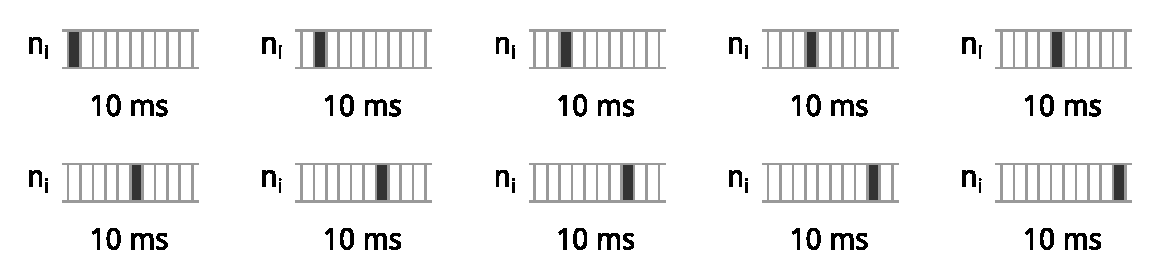
\includegraphics[width=0.9\textwidth]{spike_codes-rate-1}
    \caption{Spike rate example, all 10 examples encode the same value for they all have a 1 spike per 10 $ms$ rate}
    \label{fig:neuro:spike-rate-encoding-cap}
  \end{center}
\end{figure}

\subsection{Temporal codes}
The precise time a spike was emitted is what encodes information, this translates in a larger representation capacity. Most authors agree that a temporal resolution of $1ms$ is enough to represent the dynamics of neural networks in the brain. Although the precise time is what is theorized, it is probably not a realistic approach since spike recordings are rarely noise-free and this could alias values. Creating artificial neural networks that use temporal coding is an active field of research, in this regard, \emph{polychronization} is a promising theory for this type of neural code~\cite{polychronization-Izhikevich2005}. As with rate codes, the term temporal code is used for multiple definitions, some of which are briefly introduced next.

\subsubsection{Time-to-first-spike}
Information is encoded in the time it takes a neuron to spike after a certain temporal barrier is set (Figure \ref{fig:neuro:time-to-first}).

\subsubsection{Synchrony}
The concept behind this is that whenever neurons fire at the same time, they should be classified together. A value would be represented by different combinations of neurons firing at the same time (Figure \ref{fig:neuro:synchrony}).

\subsubsection{Phase}
The values are encoded in the phase of the spikes with respect of a background oscillating signal or rhythm (Figure \ref{fig:neuro:phase}).

\begin{figure}
  \begin{center}
  \begin{subfigure}{0.25\textwidth}
%    \vspace*{0.8em}
    \centering
    \captionsetup{justification=centering}
    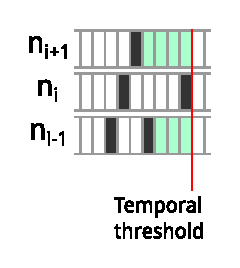
\includegraphics[width=\textwidth]{spike_codes-time-to-first}
    \caption{Time-to-first-spike}
    \label{fig:neuro:time-to-first}
  \end{subfigure}
  \begin{subfigure}{0.25\textwidth}
%    \vspace*{0.8em}
    \centering
    \captionsetup{justification=centering}
    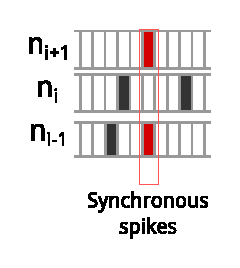
\includegraphics[width=\textwidth]{spike_codes-synchrony}
    \caption{Synchrony}
    \label{fig:neuro:synchrony}
  \end{subfigure}
  \begin{subfigure}{0.265\textwidth}
      \centering
      \captionsetup{justification=centering}
      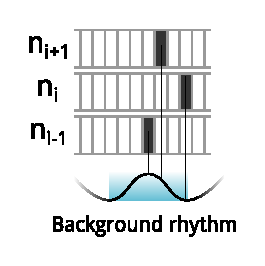
\includegraphics[width=\textwidth]{spike_codes-phase}
      \caption{Phase}
      \label{fig:neuro:phase}
  \end{subfigure}
  \caption{Different temporal codes}
  \label{fig:neuro:temporal-codes}
  \end{center}
\end{figure}

\subsubsection{Rank-order}
Using this type of encoding, only the temporal order of the spikes generated by a group of neurons is important. This means that a value is encoded in the order of a group of neurons firing.

\begin{figure}[hbt]
  \begin{center}
    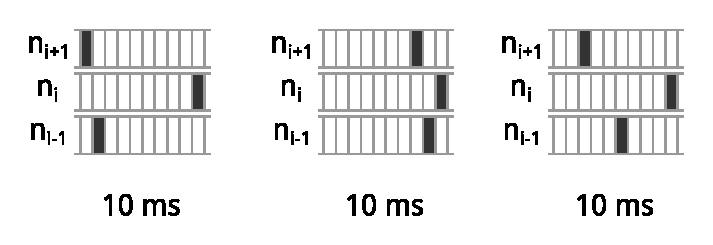
\includegraphics[width=0.65\textwidth]{spike_codes-rank}
    \caption{Rank-order example. Since all the examples have neurons firing in the same order, they all encode the same value.}
    \label{fig:neuro:spike-rank-order}
  \end{center}
\end{figure}

An issue that has been noted by some on rank-order encoded information is the fact that spike trains that are notably different (Figure \ref{fig:neuro:spike-rank-order}) are interpreted as the same value. This might be corrected by changing the metrics used to determine the uniqueness of a spike train set~\cite{Cessac2010}. On the other hand, this same issue could be seen as a robust way of encoding information.

